% intro %
\subsection{Introduction}
When particles are collided at high energies inside a particle detector, the collision products will either decay quickly into stable particles that can be detected or simply it would not interact with the detector. To able to know the products originated from collision, we need a way to reconstruct them from information gathered from the detector signals as shown in Fig.~\ref{fig:Particles_in_CMS}. 
CMS experiments is able to achieve that using a Holistic approach that was first developed by the ALEPH experiment at LEP that is called particle flow (PF).

This algorithm uses the various signals captured by the CMS subdetectors to derive physics objects originated from the collision, such as muons, electrons, photons, jets, taus, missing transverse energy, for each event.This section will provide a brief description of PF algorithm, and one of the PF elements calorimeter clusters. Additionally, calibration cluster calibration using the conventional method. %(might move to have his own section)

\subsection{Particle Flow Algorithm}
As mentioned previously, The PF algorithm aims to reconstruct and identify all final particles produce in the event ,an event is a snapchat of a collision in the LHC %source. 
This is achieved by utilizing the fact that different particles leave different signatures in the CMS subdetectors. As shown in this figure As shown in Fig.~\ref{fig:PF_diagram}

There are two types of PF algorithms: Online (in ECAL chapter we cover HLT PF cluster calibration), required to be done quickly during data taking to select interesting events and it is not integrated in the PF framework, and offline which that is done after data is collected and it takes more time to achieve higher precision. %(source about PF and HLT , source section3  )

The PF algorithm is done in multiple steps and there are advanced algorithm used to reconstruct for energy clusters and charge particles tracks,
are integrated in the PF framework. 
\begin{itemize}
\item First:it starts with reconstructing the basic elements of the PF algo: tracks, energy clusters. The details of the clustering algorithm and the calibration of the clusters will be discussed in the next sections.
  
 \item Second: forming links between the PF elements based on their spatial proximity. the linking rule is to Cannect a small thing a big one where they must be touching in the eta-phi space, the order of the size from small to big (track,Ecal cluster, Hcal cluster).
   Types of links that could be formed between:tracks and ECAL cluster, tracks and HCAL clusters, ECAL and HCAL clusters, inner tracks and muon tracks,
   muon tracks and ECAL clusters, muon tracks and HCAL clusters.
   After all the links are established, PF blocks are formed from all groups of linked tracks and clusters.
   (We could have blocks from an alone element like a single track or a cluster (insert skitch of the blocks)
   
 \item Final step in the PF is to derive the list of PF particle candidate from the PF blocks. This decision is done by following a strict order.
   After checking the tracks and clusters associated to a PF candidate, they will be removed from their blocks.
   This order starts with the cleanest signature in the CMS muons.
   Then, isolated electrons and photons (this is ECAL clusters not linked to HCAL cluster).
   After those neutral hadrons and photon (all left clusters without track link) where Ecal cluster will be assigned to photon candidates and HCAl clusters will be assigned to a neural hadron.
   Lastly everything left are charged hadrons. For charged hadrons, the energy must be calibrated. This could be done by comparing the sum of cluster energy to the sum of the track momenta. (Expand more on the calibration done here, and in case overlap of charged and neutral hadron). Also, any alone tracks will be assigned as charge hadrons. 

\end{itemize}

\subsection{Calorimeter Clustering}
Clustering in done in each calorimeter following three steps. we need to identify topological clusters and their seeds. After that we can compute cluster positions and energies.
\begin{itemize}
 \item First, we can identify topological clusters by looking for a group of calorimeter cells, each has energy deposit above a certain threshold,
   that share at least one neighbor. (include table of the threshold values in CMS calorimeter)
   
 \item Then, we identify any calorimeter cell whose energy is a local maximum, with respect to its immediate neighbors, this is a seed. Topological clusters must have one seed or multiple.
   
 \item Lastly, we compute the cluster positions and energies.we have two kinds of topological clusters.
   One with Single-seed and the other type has Multiple-seed.
   In the Single-seed case the cluster energy will be the sum of all the individual cell energies within the cluster and its position is going to be the energy-weighted average of the individual cell positions. For Multiple-seed case, each seed is assumed to represent a unique energy cluster, but the energy deposited in non-seed cells will be shared between the various clusters within the topological cluster. An iterative procedure is used to converge on cluster energies and positions based on energy-weighted averages of fractional cell energies.
 (include figures that shows topological clusters and their seeds Fig.~\ref{fig:clustering})  

\end{itemize} 


%------------ figures ------------%
% PF % 
\begin{figure}[t!]
\centering
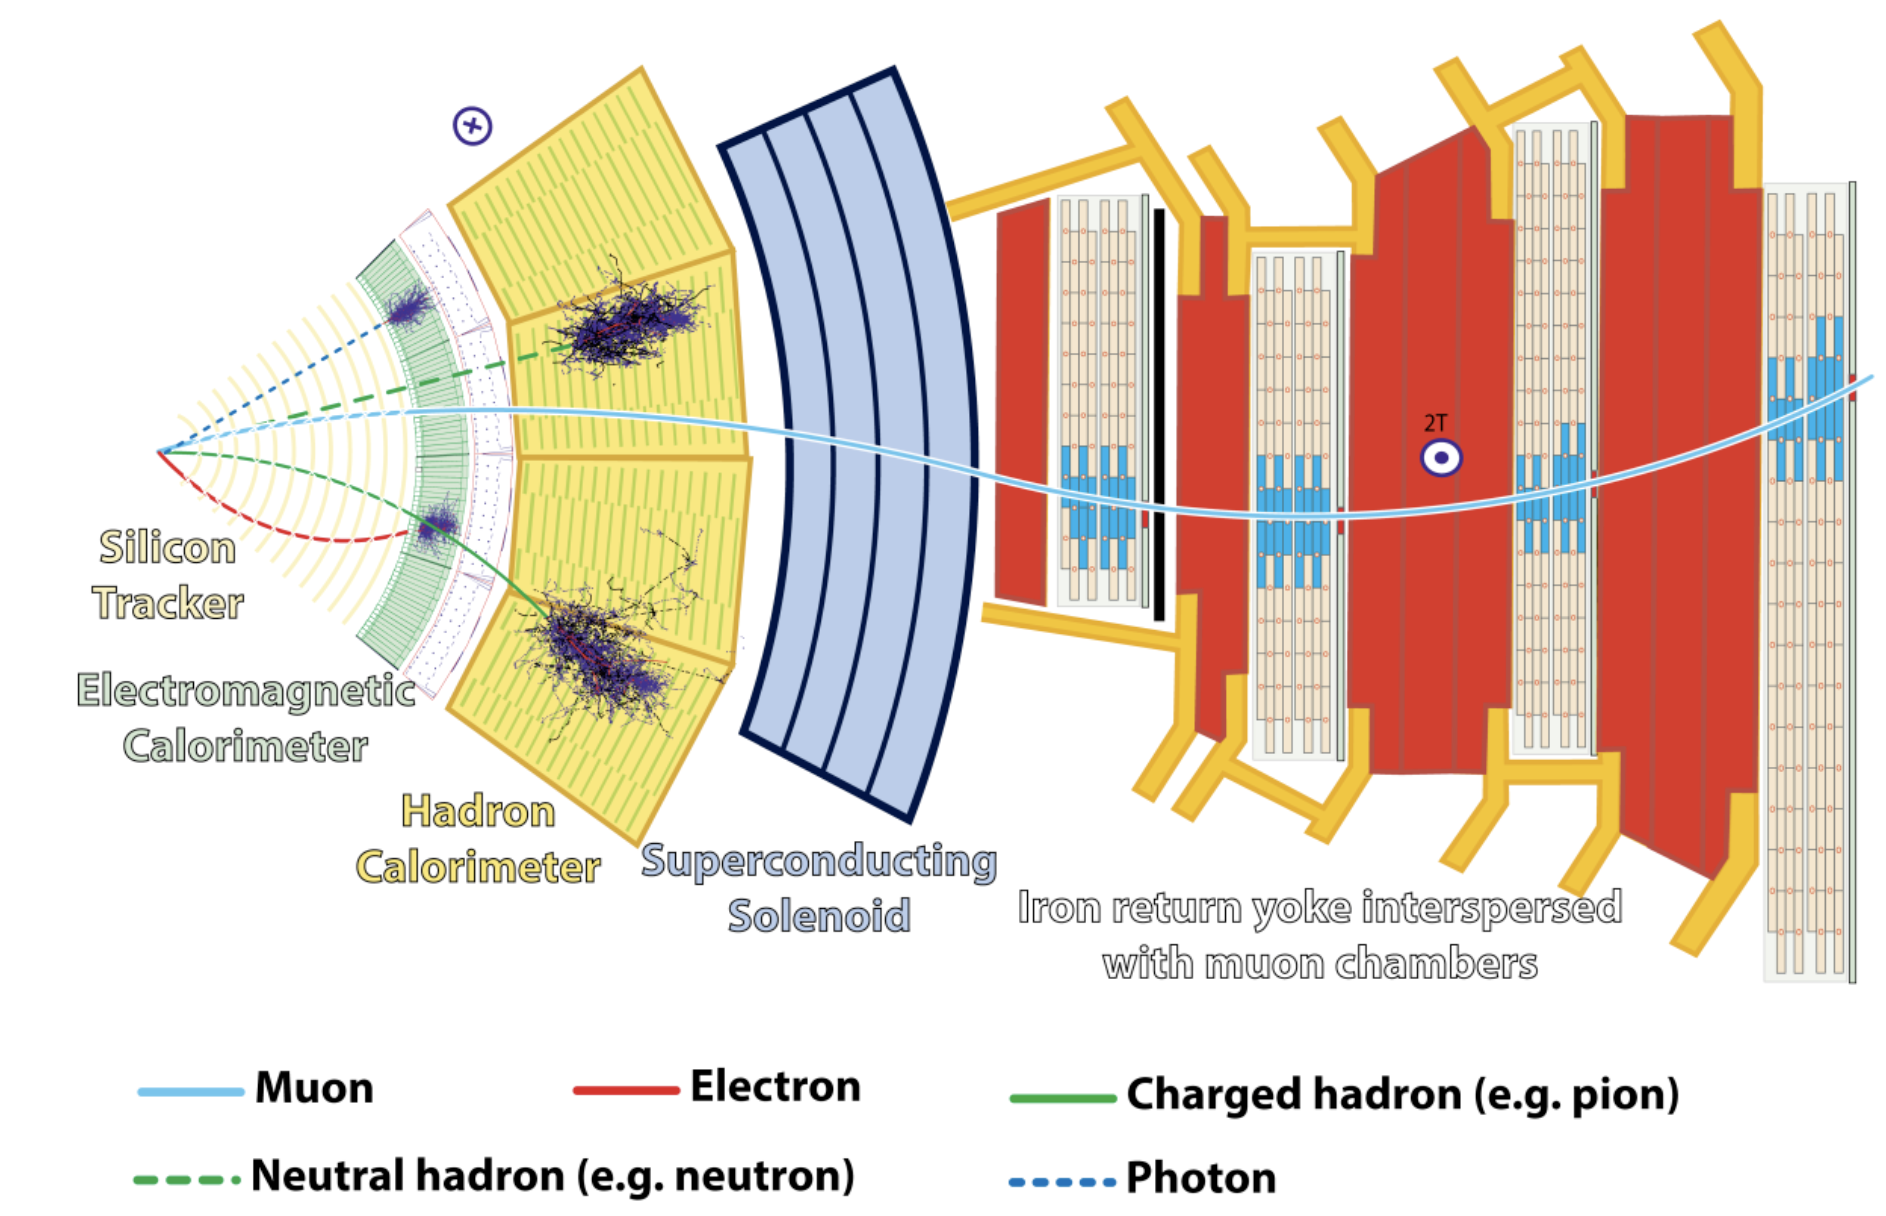
\includegraphics[width=0.99\textwidth]{figures/particles_signture_in_detector.png}
\caption[Particles signture in detector]{Particles signture in detector}. Figure source~\cite{SMtable}.                                                                        
\label{fig:Particles_in_CMS}                                                                                                               
\end{figure}

\begin{figure}[t!]
\centering
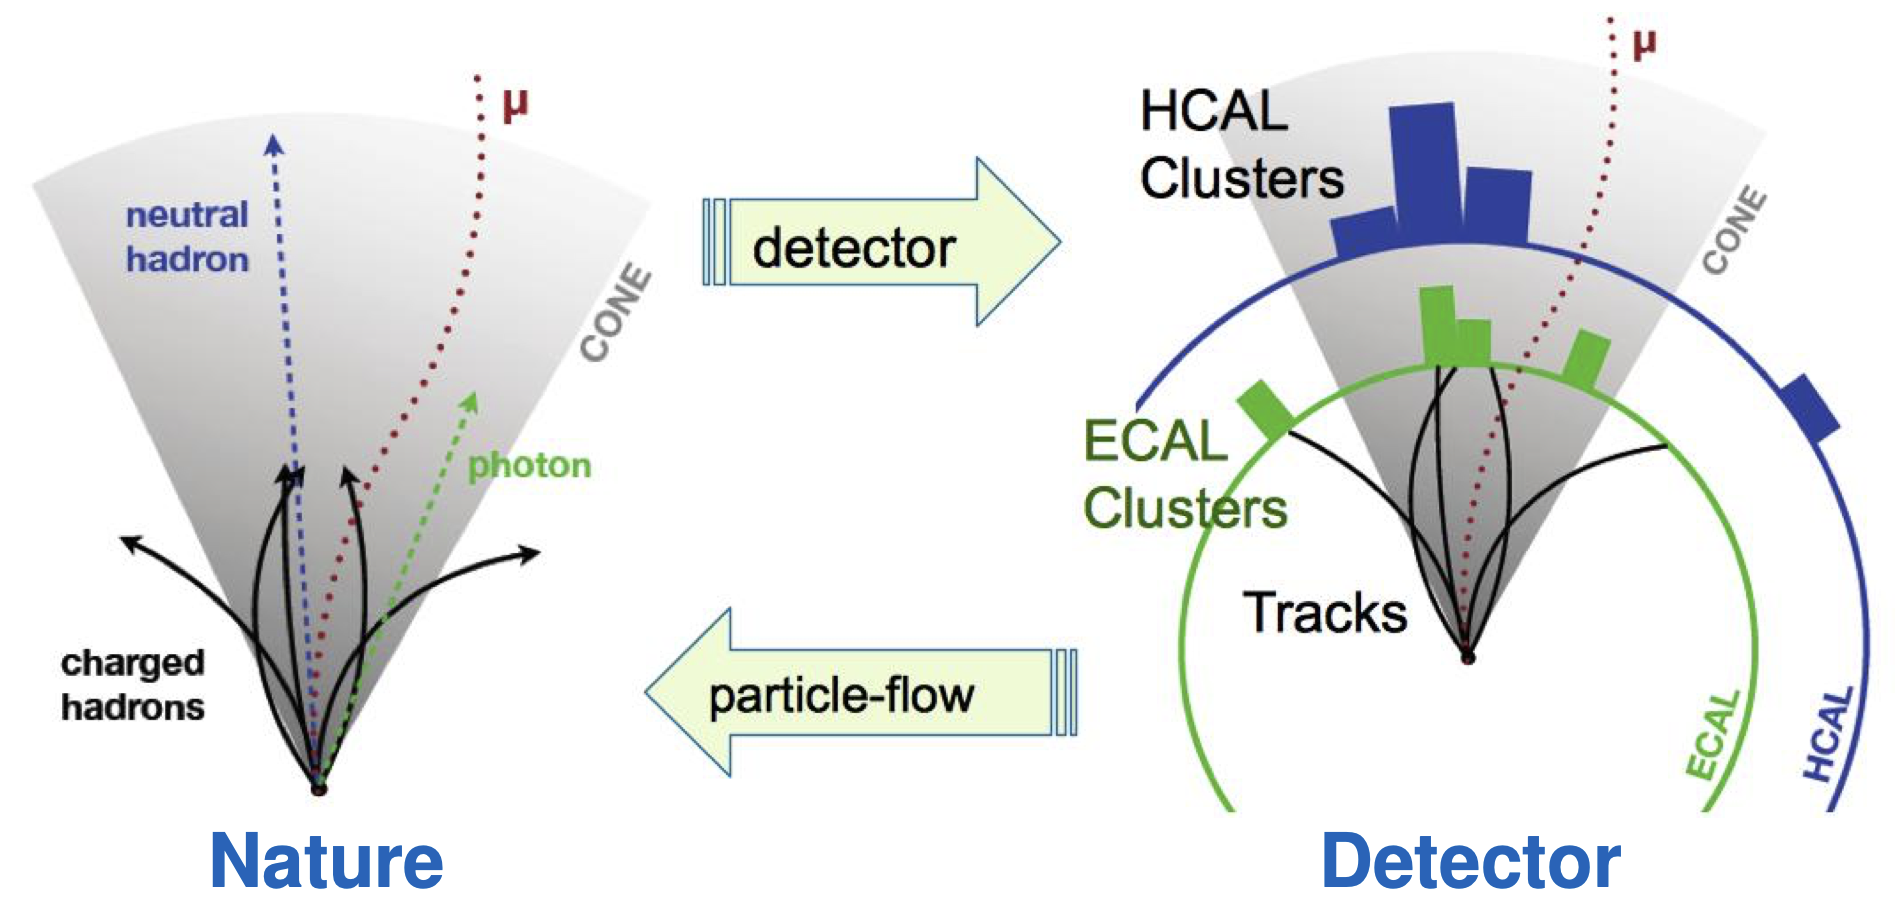
\includegraphics[width=0.99\textwidth]{figures/PF.png}
\caption[PF translate detector info]{PF translate detector info}. Figure source~\cite{SMtable}.                                                                        
\label{fig:PF_diagram}                                                                                                               
\end{figure}

% clusering %
\begin{figure}[t!]
\centering
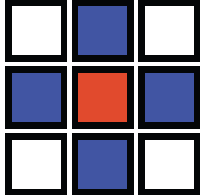
\includegraphics[width=0.25\textwidth]{figures/seed_4neighbours.png}
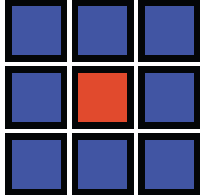
\includegraphics[width=0.25\textwidth]{figures/seed_8neighbours.png}
\caption[Different types of seeds]{Different types of seeds}. Figure source~\cite{SMtable}.                                                                        
\label{fig:seeds}}                                                                                                               
\end{figure}

\begin{figure}[t!]
\centering
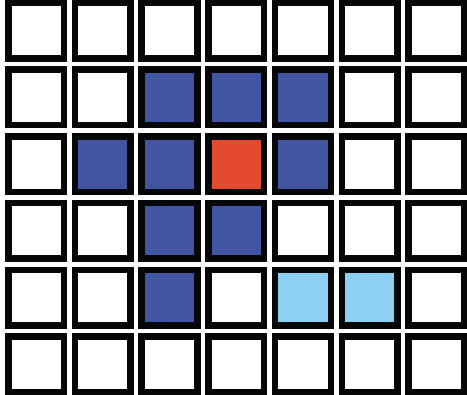
\includegraphics[width=0.25\textwidth]{figures/topological_cluster_oneseed.png}
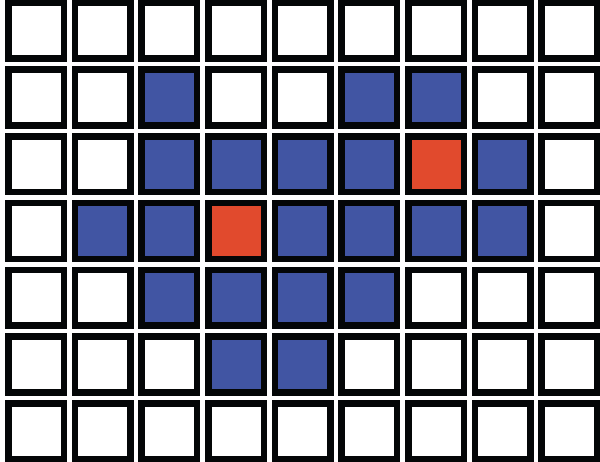
\includegraphics[width=0.25\textwidth]{figures/topological_cluster_many_Seeds.png}
\caption[Types of topological cluster]{Types of topological cluster}. Figure source~\cite{SMtable}.                                                                
\label{fig:topo_cluster}}                                                                                                               
\end{figure}

\begin{figure}[t!]
\centering
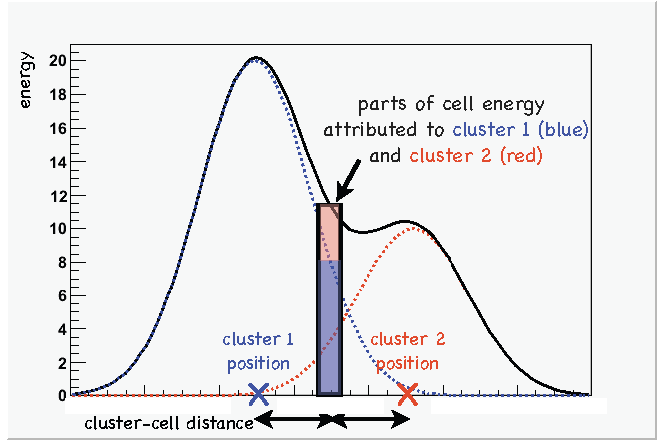
\includegraphics[width=0.50\textwidth]{figures/energy_sharing.png}
\caption[Energy shared between clusters]{Energy shared between clusters}. Figure source~\cite{SMtable}.                                                            
\label{fig:clustering}                                                                                                               
\end{figure}
